% Provenance (never printed): old terminale S material on magmatism in
% subduction zones (volcanic arcs above the slab, water released by the slab
% and hydrous melting of the mantle wedge, andesitic volcanism and granitoid
% plutons, growth of the continental crust). Owner (Sync 0): volcanic arc,
% hydrous melting, granodiorite, batholith, continental growth. Subduction,
% slab, Wadati-Benioff zone, blueschist and eclogite are g11.06's; partial and
% decompression melting and peridotite g11.05's; andesite, diorite, rhyolite,
% pluton g11.08's; continental crust g12.01's; magma, explosive eruption Book 1's
% (g7): recalled, never redefined. Figures: figdata/grade-12/arc_magmatism.py
% (GVP volcanoes, ComCat NE Japan band, dry solidus via grade-11
% geotherm_solidus.py, wet solidus brackets of Wang 2020 and Kawamoto-Holloway 1997).
\chapter{الصهارية في نطاقات الاندساس}\label{ch:g12:subduction-magmatism}

في 18 مايو 1980، عند الساعة 8:32 صباحًا، هزّ زلزال قدره 5.1
جبل سانت~هيلينز. فانزلق في الحال الجانب الشمالي للبركان، الذي كان
ينتفخ نحو الخارج بنحو مترين في اليوم: إنه أكبر انهيار ركامي
سُجّل في التاريخ، نحو \qty{2.5}{km^3} من الصخور. وإذ تحررت الصهارة الغنية بالغاز التي في الداخل من
حملها، انفجرت جانبيًا عبر الندبة، بسرعة لا تقل
عن \qty{480}{km/h}، فسوّت الغابات بالأرض على مساحة \qty{600}{km^2}. وفي غضون
خمس عشرة دقيقة ارتفع عمود من الرماد أكثر من \qty{24}{km}،
واستمر الثوران تسع ساعات. وقُتل واحد وستون شخصًا أو لم يُعثر عليهم قط.
% ledger: usgs:b2-msh-1980, usgs:msh-deaths

\begin{omfigure}
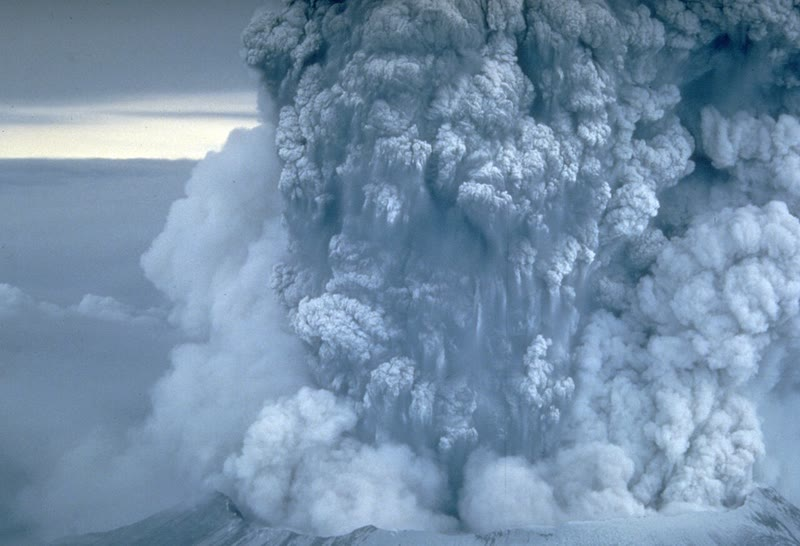
\includegraphics[width=0.55\linewidth]{images/book2/g12-swanson-st-helens-plume.jpg}

{\small عمود الرماد فوق جبل سانت~هيلينز في 18 مايو 1980، وقد ارتفع أكثر
من \qty{24}{km} في أقل من خمس عشرة دقيقة. الصورة: دونالد
أ.~سوانسون، هيئة المسح الجيولوجي الأمريكية (ملك عام).}
\end{omfigure}
% ledger: photo:g12-st-helens, usgs:b2-msh-1980

جبل سانت~هيلينز واحد من صف من البراكين --- بيكر، ورينييه، وهود،
وشاستا وغيرها --- يقوم فوق المكان الذي تغوص فيه صفيحة محيطية
صغيرة، هي صفيحة خوان دي فوكا، تحت أمريكا الشمالية. يسأل هذا الفصل
لماذا توجد البراكين هناك، ولماذا تكون ثوراناتها عنيفة في أحيان كثيرة،
وماذا يحلّ بالصهارة التي لا تبلغ السطح أبدًا.
% ledger: earle:cascades

\begin{recall}
في \omterm{def:g11:subduction-zones:subduction}{نطاق الاندساس}، تغوص صفيحة من \omterm{def:g11:ocean-ridges:oceanic-lithosphere}{الغلاف الصخري المحيطي} عائدة إلى
الوشاح تحت صفيحة أخرى؛ وزلازلها، أي \omterm{def:g11:subduction-zones:benioff}{نطاق واداتي--بينيوف}،
ترسم \omterm{def:g11:subduction-zones:slab}{اللوح المندس} نزولًا حتى عمق \qty{670}{km}
(\cref{ch:g11:subduction-zones}). والوشاح مكوّن من \omterm{def:g11:ocean-ridges:peridotite}{البيريدوتيت}؛ وهو
صلب، لكن الصخر الذي يصعد فيقل انعصاره قد ينصهر جزئيًا،
\omterm{def:g11:ocean-ridges:partial-melting}{بالانصهار بتخفيف الضغط}، كما تحت الظهرة (\cref{ch:g11:ocean-ridges}).
\omterm{def:g11:igneous-rocks:rock-names}{والأنديزيت} \omterm{def:g11:igneous-rocks:volcanic-plutonic}{صخر بركاني} وسط بين البازلت \omterm{def:g11:igneous-rocks:rock-names}{والريوليت}، \omterm{def:g11:igneous-rocks:rock-names}{والديوريت} مكافئه
الجوفي، \omterm{def:g11:igneous-rocks:intrusion}{والبلوتون} جسم كبير من الصهارة برد تحت الأرض
(\cref{ch:g11:igneous-rocks}). \omterm{def:g12:continental-crust:continental-crust}{والقشرة القارية} سميكة وخفيفة،
وأعلاها في معظمه صخر غرانيتي (\cref{ch:g12:continental-crust}). والثوران
الانفجاري يمزّق الصهارة قطعًا بغازها هي (الكتاب 1، الصف 7).
\end{recall}
% ledger: tulane:magma-types, tulane:intrusions, rg14:crust

\section{الأقواس البركانية}

معظم البراكين النشطة على اليابسة لا تقوم عشوائيًا. فمن البراكين البالغ عددها 1214
التي ثارت منذ نهاية العصر الجليدي الأخير والمدرجة
في فهرس برنامج البراكين العالمي، يقوم 838 --- أي أكثر من اثنين من كل
ثلاثة --- فوق \omterm{def:g11:subduction-zones:subduction}{نطاق اندساس}. وحول المحيط الهادئ تصنع حلقة
تكاد تكون متصلة، تُسمّى في الغالب حلقة النار، وكل صف منها
يمتد موازيًا لخندق، على جانب الصفيحة التي لا تغوص.
% values: n_volcanoes 1214, n_subduction 838, frac_subduction 0.690 (arc_magmatism.py)
% ledger: data:gvp, tulane:arc

\begin{omfigure}
\begin{tikzpicture}
\begin{axis}[ommap, width=\linewidth, xtick={-180,-90,...,180}, ytick={-60,0,60},
  legend style={font=\scriptsize, at={(0.5,-0.13)}, anchor=north, legend columns=3,
    /tikz/every even column/.append style={column sep=6pt}}]
\addplot[fill=omLithAlluv, draw=black!45, line width=0.2pt, forget plot] table {figdata/out/shared-geo-land.dat};
\addplot[black!70, line width=0.5pt, forget plot] table {figdata/out/shared-geo-school-subduction.dat};
\addplot[fill=black!70, draw=none, forget plot] table {figdata/out/shared-geo-school-teeth.dat};
% computed in figdata/grade-12/arc_magmatism.py; ledger: data:gvp, data:pb2002, data:ne-land
\addplot[only marks, mark=triangle*, mark size=1.1pt, black!40] table[x=lon, y=lat] {figdata/out/grade-12-arc_magmatism-world-other.dat};
\addplot[only marks, mark=triangle*, mark size=1.3pt, omThm] table[x=lon, y=lat] {figdata/out/grade-12-arc_magmatism-world-sub.dat};
\addlegendimage{black!70, line width=0.5pt}
\legend{{براكين أخرى}, {براكين فوق نطاق اندساس}, {خندق}}
\end{axis}
\end{tikzpicture}

{\small البراكين النشطة منذ نهاية العصر الجليدي الأخير، بالأحمر حيث
تقوم فوق \omterm{def:g11:subduction-zones:subduction}{نطاق اندساس}، مع الخنادق (خط أسود، والمثلثات
على الصفيحة الراكبة). البيانات: برنامج البراكين العالمي لمؤسسة سميثسونيان؛
وحدود الصفائح من بيرد (2003)؛ واليابسة من \babelsublr{Natural Earth}.}
\end{omfigure}
% values: n_subduction 838 of 1214 (arc_magmatism.py)

\begin{definition}[القوس البركاني]\label{def:g12:subduction-magmatism:arc}
\emph{القوس البركاني}\index{قوس بركاني} صف من البراكين على
الصفيحة الراكبة في \omterm{def:g11:subduction-zones:subduction}{نطاق اندساس}، موازٍ للخندق، قائم
فوق المكان الذي بلغ فيه \omterm{def:g11:subduction-zones:slab}{اللوح المندس} عمقًا قدره نحو مئة
كيلومتر. وهو \emph{قوس جزري} حين ينهض من قاع البحر، كما
في اليابان أو إندونيسيا، وقوس قاري حين يقوم على قارة،
كما في الأنديز أو سلسلة كاسكيد.
\end{definition}
% ledger: tulane:arc, earle:arc-water, earle:cascades, sa06:slab-depth

تُسمّى حافة القوس الأقرب إلى الخندق \textbf{الجبهة
البركانية}: فعلى جانبها المواجه للخندق لا توجد براكين أصلًا. فما عمق
\omterm{def:g11:subduction-zones:slab}{اللوح المندس} تحتها؟

\begin{proposition}[اللوح المندس تحت الجبهة البركانية]\label{prop:g12:subduction-magmatism:depth}
إذا كان \omterm{def:g11:subduction-zones:slab}{اللوح المندس} مستويًا يميل بزاوية $\theta$ انطلاقًا من الخندق،
وكانت الجبهة البركانية على مسافة أفقية $d$ من الخندق، فإن
أعلى \omterm{def:g11:subduction-zones:slab}{اللوح المندس} يقع تحت الجبهة على عمق
\[
  H = d \tan\theta .
\]
\end{proposition}

\begin{proof}
خذ مقطعًا رأسيًا عبر الخندق. \omterm{def:g11:subduction-zones:slab}{فاللوح المندس} والسطح
والخط الرأسي تحت الجبهة تصنع مثلثًا قائمًا، زاويته القائمة
تحت الجبهة: الضلع الممتد على السطح $d$، والضلع الرأسي
$H$، والزاوية عند الخندق $\theta$. إذن $\tan\theta = H/d$.
\end{proof}

قاست دراسة جامعة شملت 839 مركزًا \omterm{def:g11:igneous-rocks:volcanic-plutonic}{بركانيًا} على امتداد \qty{33000}{km} من الأقواس
العمق $H$ تحت كل منها: فإذا أُخذ المتوسط على مقاطع من الأقواس طولها \qty{500}{km}،
تراوح بين 72 و\qty{173}{km}، بمتوسط قدره \qty{105}{km}. فالأقواس التي فوق
\omterm{def:g11:subduction-zones:slab}{ألواح مندسة} شديدة الميل تقع قريبة من خندقها، والأقواس التي فوق \omterm{def:g11:subduction-zones:slab}{ألواح} خفيفة الميل بعيدة
عنه، لكن \omterm{def:g11:subduction-zones:slab}{اللوح المندس} تحتها يكون دائمًا على عمق نحو مئة كيلومتر.
% ledger: sa06:slab-depth

\begin{method}[إيجاد اللوح المندس تحت بركان]\label{met:g12:subduction-magmatism:slab}
\begin{enumerate}
  \item خذ زلازل شريط ضيق يعبر القوس، وارسم
        أعماقها بدلالة مسافاتها عبره، بمقياس رسم حقيقي.
  \item احتفظ بالزلازل الأعمق من نحو \qty{70}{km}: فالأضحل منها
        يقع أيضًا في الصفيحة الراكبة وعلى الصدع الفاصل بين
        الصفيحتين.
  \item ارسم الخط، أو اقرأ العمق، للزلازل العميقة تحت
        الجبهة البركانية: فذلك هو عمق \omterm{def:g11:subduction-zones:slab}{اللوح المندس} هناك.
  \item تحقق منه بالعلاقة $H = d\tan\theta$، بقياس $d$ من الخندق
        والميل $\theta$ على المقطع.
\end{enumerate}
\end{method}

\begin{omfigure}
\begin{tikzpicture}
\begin{axis}[omsection, name=jp, scale only axis, width=0.8\linewidth, height=0.2857\linewidth,
  xmin=0, xmax=700, ymin=0, ymax=250, y dir=reverse,
  xlabel={\foreignlanguage{arabic}{المسافة شرق خط الطول \babelsublr{\ang{138}} \babelsublr{(\unit{km})}}}, ylabel={\foreignlanguage{arabic}{العمق \babelsublr{(\unit{km})}}},
  xtick={0,100,...,700}, ytick={0,50,...,250}, tick label style={font=\small},
  every axis label/.append style={font=\small}]
% computed in figdata/grade-12/arc_magmatism.py; ledger: data:b2-usgs-ne-japan, data:gvp, data:pb2002
\addplot[only marks, mark=*, mark size=0.55pt, black!35] table[x=x_km, y=depth] {figdata/out/grade-12-arc_magmatism-jp-quakes.dat};
\addplot[omDef, line width=0.9pt, dashed] table[x=x_km, y=depth] {figdata/out/grade-12-arc_magmatism-jp-slab.dat};
\addplot[only marks, mark=triangle*, mark size=2.6pt, omThm] table[x=x_km, y expr=-7] {figdata/out/grade-12-arc_magmatism-jp-volc.dat};
\draw[omThm, densely dotted, line width=0.8pt] (axis cs:259.2,0) -- (axis cs:259.2,98.2);
\fill[omThm] (axis cs:259.2,98.2) circle (1.6pt);
\coordinate (front) at (axis cs:259.2,-14);
\coordinate (trench) at (axis cs:528.9,-14);
\coordinate (H) at (axis cs:262,60);
\coordinate (slab) at (axis cs:95,228);
\draw[black, line width=0.9pt] (axis cs:528.9,-12) -- (axis cs:528.9,0);
\end{axis}
\node[font=\scriptsize, anchor=south, text=omThm] at (front) {\foreignlanguage{arabic}{الجبهة البركانية: إيواتي}};
\node[font=\scriptsize, anchor=south] at (trench) {خندق اليابان};
\node[font=\scriptsize, anchor=west, text=omThm, fill=white, inner sep=1pt] at (H) {\qty{98}{km}};
\node[font=\scriptsize, anchor=west, text=omDef, fill=white, inner sep=1pt] at (slab) {\foreignlanguage{arabic}{لوح مندس يميل نحو \babelsublr{\ang{20}}}};
\end{tikzpicture}

{\small مقطع عبر شمال شرق اليابان بمقياس رسم حقيقي: الزلازل التي
قدرها 4.5 أو أكثر بين \ang{37.5} و\ang{40.5} شمالًا، 1976--2025 (بالرمادي)،
وبراكين الشريط نفسه (مثلثات حمراء) والخط الملائم
للزلازل الأعمق من \qty{70}{km} (أزرق، متقطع). واثنان من كل خمسة من
الأحداث الضحلة شرق \ang{141.5} شرقًا تعود إلى عام 2011، عام
زلزال مارس الكبير. البيانات: فهرس الزلازل لهيئة المسح الجيولوجي
الأمريكية؛ وبرنامج البراكين العالمي لمؤسسة سميثسونيان؛ وحدود الصفائح
من بيرد (2003).}
\end{omfigure}
% values: shallow (<70 km) events east of 141.5 E: 3622, of which 1451 in 2011 (0.40); ledger usgs:tohoku
% values: jp_front_lon 141.0 (x 259.2 km), jp_trench_lon 144.12 (x 528.9), jp_front_trench_km 269.4, jp_dip_deg 19.98, jp_H_geom 98.0, bin_141_median 98.15, jp_slab_depth_front 105.6 (arc_magmatism.py)

\begin{example}[شمال شرق اليابان]\label{ex:g12:subduction-magmatism:japan}
في شريط الشكل، أقصى البراكين شرقًا هو إيواتي، عند \ang{141.0} شرقًا،
ويقع خندق اليابان عند \ang{144.1} شرقًا. ودرجة الطول الواحدة هناك
$111.2\cos\ang{39} \approx \qty{86.4}{km}$، إذن $d \approx 3.12 \times 86.4
\approx \qty{270}{km}$. وتميل الزلازل العميقة بنحو \ang{20}، ومن ثم
\[
  H = 270 \times \tan\ang{20} \approx \qty{98}{km}.
\]
والزلازل الأعمق من \qty{70}{km} الواقعة تحت الجبهة نفسها
عمقها الوسيط \qty{98}{km}: فالقيمتان متفقتان، وقريبتان من المتوسط
العالمي.
\end{example}
% values: km_per_deg_lon 86.415, jp_front_trench_km 269.4, jp_dip_deg 19.98, jp_H_geom 97.98, bin_141_median 98.15 (arc_magmatism.py)

\section{الماء يصهر الوشاح}

تحت القوس، يكون \omterm{def:g11:subduction-zones:slab}{اللوح المندس} باردًا، وكذلك \omterm{def:g11:ocean-ridges:oceanic-lithosphere}{القشرة المحيطية} التي فوقه:
فلا يمكن أن تنصهر. فلا بد أن تأتي الصهارة من الوشاح الساخن الذي فوق \omterm{def:g11:subduction-zones:slab}{اللوح المندس}،
أي \textbf{إسفين الوشاح}. لكن الإسفين لا يصعد، فلا يمكن أن ينصهر بتخفيف
الضغط كما يحدث تحت الظهرة. فشيء آخر يخفض درجة حرارة
انصهاره: إنه الماء.
% ledger: earle:settings (subducted crust stays cool), earle:flux-melting, earle:arc-water

تتشبع \omterm{def:g11:ocean-ridges:oceanic-lithosphere}{القشرة المحيطية} بماء البحر قرب الظهرة التي تتكوّن عندها،
وينتهي كثير من ذلك الماء محبوسًا داخل معادنها، وأهمها
السربنتين، المصنوع من أوليفين القشرة وبيروكسينها. وكلما غاص \omterm{def:g11:subduction-zones:slab}{اللوح المندس}
وسخن، تفككت هذه المعادن وأطلقت ماءها.
فيصعد الماء إلى \omterm{def:g11:ocean-ridges:peridotite}{البيريدوتيت} الساخن في الإسفين الذي فوقه.
% ledger: earle:arc-water, tulane:arc

\begin{definition}[الانصهار المائي]\label{def:g12:subduction-magmatism:hydrous-melting}
\emph{الانصهار المائي}\index{انصهار مائي} (أو الانصهار بإضافة الماء) هو
\omterm{def:g11:ocean-ridges:partial-melting}{الانصهار الجزئي} لصخر بسبب إضافة الماء، الذي يخفض
درجة الحرارة التي يبدأ عندها الصخر بالانصهار.
\end{definition}
% ledger: earle:flux-melting, earle:arc-water

درجة الحرارة التي يبدأ عندها صخر بالانصهار، تحت ضغط معين، هي
\textbf{خط تصلبه}. وهو معروف جيدًا \omterm{def:g11:ocean-ridges:peridotite}{للبيريدوتيت} الجاف؛ أما مع الماء فقياسه
أصعب بكثير، ولا تزال القيم المنشورة تختلف بمقدار 200 إلى
\qty{600}{\celsius}. وأحدث التجارب تضعه بين 950
و\qty{1000}{\celsius} عند \qty{3}{GPa}، أي على عمق نحو \qty{95}{km}، وفوق
\qty{1000}{\celsius} بقليل من 5 إلى \qty{11}{GPa}. أما \omterm{def:g11:ocean-ridges:peridotite}{البيريدوتيت} الجاف عند \qty{3}{GPa}
فلا يبدأ بالانصهار إلا عند نحو \qty{1470}{\celsius}: فالماء يخفض خط التصلب
بنحو \qty{500}{\celsius}.
% values: dry_T_3gpa 1473.4, dry_minus_wet_3gpa 498, z_3gpa_km 95.2, dry_minus_wet_5gpa 658 (arc_magmatism.py)
% ledger: hirschmann:solidus, wang20:wet-solidus, kh97:wet-solidus, data:prem, earth:gmean

\begin{omfigure}
\begin{tikzpicture}
\begin{axis}[omrecord, name=sol, scale only axis, width=0.62\linewidth, height=6.2cm,
  xmin=700, xmax=1900, ymin=0, ymax=230, y dir=reverse,
  xlabel={\foreignlanguage{arabic}{درجة الحرارة \babelsublr{(\unit{\celsius})}}}, ylabel={\foreignlanguage{arabic}{العمق \babelsublr{(\unit{km})}}},
  xtick={800,1000,...,1800}, ytick={0,50,...,200}, axis y line*=left]
% computed in figdata/grade-12/arc_magmatism.py (dry: Hirschmann 2000 with PREM pressures; wet: Wang 2020, Kawamoto-Holloway 1997)
\addplot[omProp, line width=1.2pt] table[x=T_dry, y=depth_km] {figdata/out/grade-12-arc_magmatism-solidus.dat};
\addplot[omDef, line width=2.4pt] coordinates {(950,95.24) (1000,95.24)};
\addplot[omDef, line width=1.2pt] coordinates {(1000,155.6) (1000,216.3)};
\draw[-{Stealth}, black!70, line width=0.8pt] (axis cs:1460,95.24) -- (axis cs:1015,95.24);
\coordinate (gap) at (axis cs:1240,95.24);
\coordinate (dry) at (axis cs:1600,40);
\coordinate (wet) at (axis cs:1015,190);
\coordinate (wet3) at (axis cs:975,90);
\end{axis}
\begin{axis}[scale only axis, width=0.62\linewidth, height=6.2cm, at={(sol.south west)}, anchor=south west,
  xmin=700, xmax=1900, ymin=0, ymax=230, y dir=reverse, axis x line=none, axis y line*=right,
  axis line style={-}, ylabel={\foreignlanguage{arabic}{الضغط \babelsublr{(\unit{GPa})}}},
  ytick={34.9,65.1,95.2,125.5,155.6,185.9,216.3}, yticklabels={1,2,3,4,5,6,7},
  every axis label/.append style={font=\small}, tick label style={font=\small}]
% pressure ticks at the PREM depths of 1-7 GPa (arc_magmatism.depth_at_pressure)
\end{axis}
\node[font=\scriptsize, anchor=south] at ([yshift=2pt]gap) {\foreignlanguage{arabic}{نحو \babelsublr{\qty{500}{\celsius}}}};
\node[font=\scriptsize, text=omProp, anchor=west, align=left] at (dry) {بيريدوتيت جاف\\يبدأ بالانصهار};
\node[font=\scriptsize, text=omDef, anchor=west, align=left] at (wet) {\foreignlanguage{arabic}{مع الماء: فوق}\\\foreignlanguage{arabic}{\babelsublr{\qty{1000}{\celsius}} بقليل}};
\node[font=\scriptsize, text=omDef, anchor=south] at ([yshift=2pt]wet3) {950--1000};
\end{tikzpicture}

{\small درجة الحرارة التي يبدأ عندها \omterm{def:g11:ocean-ridges:peridotite}{بيريدوتيت} الوشاح بالانصهار، بدلالة
العمق: جافًا (بالبرتقالي) ومشبعًا بالماء (بالأزرق، المجالان المقيسان
حتى الآن). وعند عمق \omterm{def:g11:subduction-zones:slab}{اللوح المندس} تحت الأقواس، نحو \qty{100}{km}، يخفضها
الماء بنحو \qty{500}{\celsius}. المصادر: هيرشمان (2000)، مع
كثافات \babelsublr{PREM}؛ ووانغ وآخرون (2020)؛ وكاواموتو وهولوواي (1997).}
\end{omfigure}
% values: dry_T_3gpa 1473.4, dry_T_100km 1489.4, P_100km_gpa 3.157 (arc_magmatism.py)

وهكذا يفعل الماء ما لم يكن التسخين وحده ليفعله: يجعل جزءًا من الإسفين
الساخن ينصهر. فتصعد الصهارة، الأخف من الوشاح الصلب المحيط بها،
نحو السطح؛ فيثور بعضها، ويبقى أكثرها ويبرد تحت الأرض.
والمكان الذي يتحرر فيه الماء، والذي يكون الإسفين فوقه ساخنًا بما يكفي
لينصهر ما إن يبتل، هو ما يثبّت الجبهة البركانية على ارتفاع نحو مئة كيلومتر
فوق \omterm{def:g11:subduction-zones:slab}{اللوح المندس}.
% ledger: earle:arc-water, tulane:arc, sa06:slab-depth, wang20:wet-solidus (position of the volcanic front controlled by melting in the wedge)

\begin{omfigure}
\begin{tikzpicture}[x=1cm, y=1cm, font=\scriptsize]
  % mantle
  \fill[omLithPeridotite!45] (0,-0.9) -- (7.4,-0.9) -- (7.5,-0.85) -- (6.5,-1.6) -- (5.5,-2.6) -- (4.5,-3.8)
    -- (4.25,-4.3) -- (0,-4.3) -- cycle;
  % sea and overriding continental crust
  \fill[omSea] (8.0,0) -- (12,0) -- (12,-0.4) -- (8.5,-0.4) -- cycle;
  \fill[omLithGranite!55] (0,0.1) -- (8.0,0.1) -- (8.5,-0.4) -- (7.5,-0.85) -- (7.4,-0.9) -- (0,-0.9) -- cycle;
  % the slab
  \fill[omLithBasalt!45, draw=black!60] (12,-0.4) -- (8.5,-0.4) -- (7.5,-0.85) -- (6.5,-1.6) -- (5.5,-2.6) -- (4.5,-3.8)
    -- (4.25,-4.3) -- (5.15,-4.3) -- (5.2,-4.3) -- (6.15,-3.15) -- (7.1,-2.2) -- (8.0,-1.55) -- (8.9,-1.2) -- (12,-1.2) -- cycle;
  \node at (10.4,-0.8) {غلاف صخري محيطي};
  \node[anchor=west] at (6.0,-3.4) {لوح مندس غائص};
  % melting in the wedge, rising magma, plutons, volcano
  \fill[omThm!35, draw=omThm, densely dashed] (5.2,-1.75) ellipse (0.6 and 0.3);
  \node[omThm] at (5.2,-1.75) {انصهار};
  \foreach \y in {-1.3,-1.05} \fill[omThm!80] (5.2,\y) circle (0.07);
  \fill[omLithGranite, draw=black!60] (4.75,-0.55) ellipse (0.42 and 0.2);
  \fill[omLithGranite, draw=black!60] (5.65,-0.4) ellipse (0.32 and 0.16);
  \node[anchor=east] at (4.25,-0.55) {بلوتونات};
  \draw[omThm, line width=1pt] (5.2,0.1) -- (5.2,-0.85);
  \fill[black!65] (4.75,0.1) -- (5.2,0.75) -- (5.65,0.1) -- cycle;
  \node[anchor=south] at (5.2,0.8) {بركان};
  % water released by the slab
  \foreach \x/\y in {6.5/-1.6, 6.0/-2.1, 5.6/-2.5}
    \draw[omDef, -{Stealth}, line width=0.7pt, decorate, decoration={snake, amplitude=0.6pt, segment length=4pt, post length=1.5mm}]
      (\x,\y) -- ++(-0.3,0.3);
  \draw[omDef, line width=0.3pt] (7.5,-2.75) -- (6.35,-2.0);
  \node[omDef, anchor=west, align=left] at (7.5,-2.75) {ماء يحرره\\اللوح المندس};
  % labels and depth scale
  \node at (1.8,-0.4) {قشرة قارية};
  \node[black!70, align=center] at (2.3,-3.6) {إسفين وشاح ساخن\\(بيريدوتيت)};
  \node[anchor=south] at (8.5,0.12) {خندق};
  \draw[black!60, |-|] (0.4,0.1) -- node[left, align=right] {نحو\\\babelsublr{\qty{100}{km}}} (0.4,-2.96);
  \draw[black!45, densely dotted] (0.4,-2.96) -- (5.2,-2.96);
  \fill[black!70] (5.2,-2.96) circle (1.3pt);
  \draw[black!45, densely dotted] (5.2,-2.96) -- (5.2,-2.05);
\end{tikzpicture}

{\small الصهارية في \omterm{def:g11:subduction-zones:subduction}{نطاق اندساس} (رسم تخطيطي، ليس بمقياس رسم حقيقي). كلما سخن \omterm{def:g11:subduction-zones:slab}{اللوح المندس}،
أطلقت معادنه ماءها، فيصعد إلى إسفين الوشاح الساخن
ويجعله ينصهر جزئيًا. وتصعد الصهارة: فيثور بعضها عند
البراكين، ويبرد أكثرها في القشرة على هيئة \omterm{def:g11:igneous-rocks:intrusion}{بلوتونات}.}
\end{omfigure}
% ledger: earle:arc-water, earle:flux-melting, tulane:arc, tulane:ridge-rocks, sa06:slab-depth

\section{الأنديزيت والغرانوديوريت}

الصهارات الأولى \omterm{def:g11:ocean-ridges:peridotite}{للبيريدوتيت} الرطب ليست بازلتية. ففي تجارب عند
\qty{1}{GPa}، يعطي \omterm{def:g11:ocean-ridges:peridotite}{البيريدوتيت} المشبع بالماء صهارات ذات تركيب
أنديزيتي. والصهارات، وهي تصعد عبر القشرة السميكة للقوس، تتغير أيضًا كلما
بردت، من البازلتية نحو الأنديزيتية والريوليتية. ولذلك تكون صهارات الأقواس
أغنى بالسيليكا من بازلت الظهرات --- فالصهارة الأنديزيتية
تحوي منها 55 إلى \qty{65}{\percent} --- وتحمل الماء الذي صنعها.
% ledger: kh97:wet-solidus (andesitic melts at 1 GPa), tulane:eruptions, tulane:ridge-rocks, tulane:magma-types

كلتا الخاصيتين تجعل ثوراناتها عنيفة. فكلما زادت السيليكا في الصهارة،
زادت لزوجتها، وصعب على غازها أن يفلت؛ والثورانات
الانفجارية تحابيها نسبة الغاز العالية واللزوجة العالية، كما في
الصهارات الأنديزيتية والريوليتية. وتكاد البراكين المركبة كلها تقوم فوق
نطاقات \omterm{def:g11:subduction-zones:subduction}{الاندساس}: مخاريط يبلغ ارتفاعها آلاف الأمتار وعرضها ما يصل إلى \qty{20}{km}،
ومنحدراتها من 10 إلى 30 درجة، وتتراوح ثوراناتها بين مسيلات لابية
هادئة وانفجارات. وتحت جبل سانت~هيلينز، تمتد حجرة صهارية عرضها نحو \qty{1}{km}
من عمق نحو 6 إلى \qty{14}{km}.
% ledger: tulane:magma-types, tulane:eruptions, earle:composite

معظم صهارة الأقواس لا يثور أبدًا. فهو يبرد ببطء في القشرة ويتبلور
صخورًا خشنة الحبيبات.

\begin{definition}[الغرانوديوريت]\label{def:g12:subduction-magmatism:granodiorite}
\emph{الغرانوديوريت}\index{غرانوديوريت} \omterm{def:g11:igneous-rocks:volcanic-plutonic}{صخر جوفي} خشن الحبيبات
يشبه الغرانيت، لكن البلاجيوكليز فيه أكثر من فلسبار البوتاسيوم: فمن 20 إلى
\qty{60}{\percent} من معادنه الفاتحة كوارتز، ومن 65 إلى
\qty{90}{\percent} من فلسباره بلاجيوكليز؛ وكثيرًا ما يحوي البيوتيت
أو الهورنبلند.
\end{definition}
% ledger: bgs:granodiorite

\begin{omfigure}
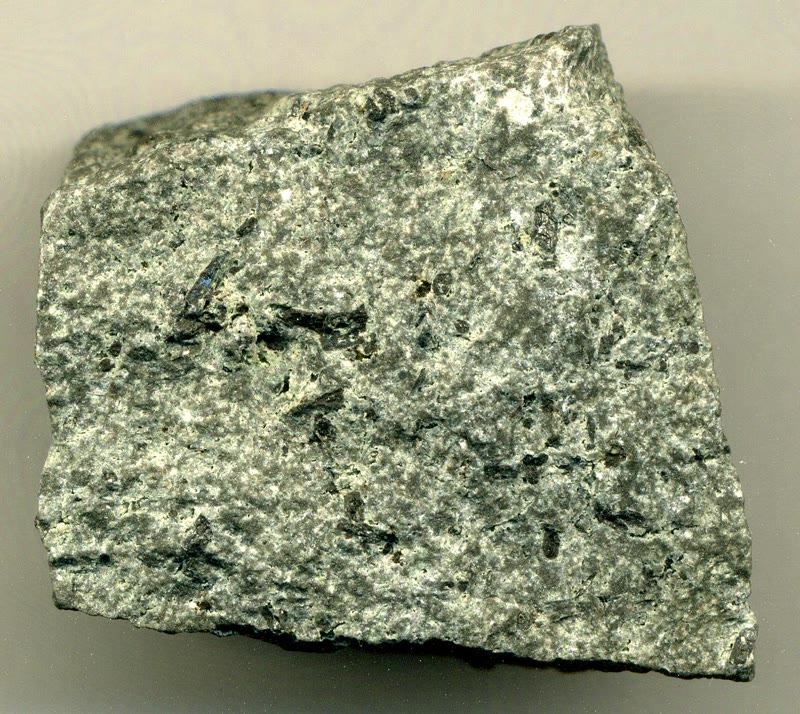
\includegraphics[height=4.4cm]{images/book2/g12-stjohn-andesite.jpg}\hspace{0.03\linewidth}%
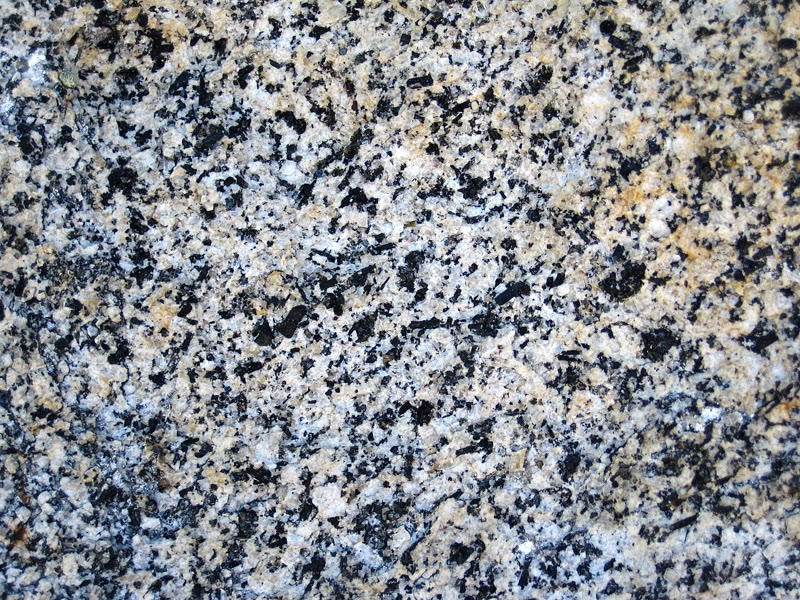
\includegraphics[height=4.4cm]{images/book2/g12-stjohn-granodiorite.jpg}

{\small في اليمين: \omterm{def:g11:igneous-rocks:rock-names}{أنديزيت}، \omterm{def:g11:igneous-rocks:volcanic-plutonic}{صخر بركاني} دقيق الحبيبات من الأقواس. في اليسار:
\omterm{def:g12:subduction-magmatism:granodiorite}{غرانوديوريت} من سييرا نيفادا، فيه بلاجيوكليز أبيض وكوارتز رمادي
وبيوتيت وهورنبلند أسودان. الصور: جيمس سانت~جون (\babelsublr{CC~BY~2.0}).}
\end{omfigure}
% ledger: photo:g12-andesite, photo:g12-granodiorite

تحوي \omterm{def:g12:continental-crust:continental-crust}{القشرة القارية} العليا في المتوسط نحو \qty{67}{\percent} من
\ce{SiO2}: فهي \omterm{def:g11:igneous-rocks:felsic-mafic}{فلسية}، كالغرانيت الذي تصنعه الأقواس بكميات كبيرة في
باثوليثاتها.
% ledger: rg14:crust (upper crust SiO2 66.6 wt %), tulane:magma-types, tulane:intrusions

\begin{definition}[الباثوليث]\label{def:g12:subduction-magmatism:batholith}
\emph{الباثوليث}\index{باثوليث} كتلة كبيرة من \omterm{def:g11:igneous-rocks:volcanic-plutonic}{الصخر الجوفي} تغطي
أكثر من \qty{100}{km^2} حيث كشفتها التعرية. ويتكوّن حيث تلتحم \omterm{def:g11:igneous-rocks:intrusion}{بلوتونات}
كثيرة، تداخلت واحدًا بعد آخر، تحت السطح.
\end{definition}
% ledger: earle:batholith, tulane:intrusions

من أكبرها في العالم المعقد الجوفي الساحلي، الذي يمتد على امتداد
ساحل المحيط الهادئ من منطقة فانكوفر في غرب كندا إلى
جنوب شرق ألاسكا. وتكوّن \omterm{def:g12:subduction-magmatism:batholith}{باثوليث} سييرا نيفادا في كاليفورنيا فوق
\omterm{def:g11:subduction-zones:subduction}{نطاق اندساس}؛ ومعظم غرانيتاته في يوسميتي تبلور في
الطباشيري، قبل 105 إلى 85 مليون سنة. وقد بُليت الصخور التي فوقها
على مدى ملايين السنين، فصارت \omterm{def:g11:igneous-rocks:intrusion}{البلوتونات} التي بردت في العمق تشكّل الآن
الجبال.
% ledger: earle:batholith, nps:yosemite, photo:g12-sierra-nevada (St. John description), ics:base.Cretaceous

\begin{omfigure}
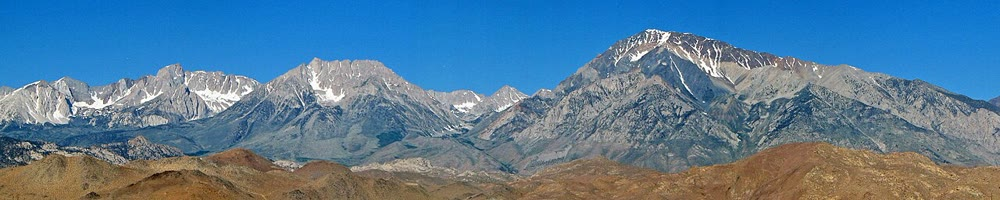
\includegraphics[width=0.94\linewidth]{images/book2/g12-stjohn-sierra-nevada-batholith.jpg}

{\small سييرا نيفادا، كما تُرى من الشرق: غرانيت \omterm{def:g12:subduction-magmatism:granodiorite}{وغرانوديوريت}
\omterm{def:g12:subduction-magmatism:batholith}{باثوليث} سييرا نيفادا، الذي تبلور في العمق فوق
\omterm{def:g11:subduction-zones:subduction}{نطاق اندساس} في الطباشيري. الصورة: جيمس سانت~جون
(\babelsublr{CC~BY~2.0}).}
\end{omfigure}
% ledger: photo:g12-sierra-nevada, nps:yosemite

\section{كيف تنمو القارات}

\begin{definition}[نمو القارات]\label{def:g12:subduction-magmatism:continental-growth}
\emph{نمو القارات}\index{نمو القارات} هو إضافة \omterm{def:g12:continental-crust:continental-crust}{قشرة قارية}
جديدة، مصنوعة من الوشاح، بصهارية الأقواس في الغالب.
والنمو الصافي للقارات هو تلك الإضافة مطروحًا منها \omterm{def:g12:continental-crust:continental-crust}{القشرة القارية}
التي تعود إلى الوشاح.
\end{definition}
% ledger: sv09:growth, ss09:balance

الأقواس هي حيث يُصنع صخر القارات الخفيف. وتقديرات
الصهارة التي تضيفها الأقواس اليوم نحو \qty{1.5}{km^3} في السنة في الأقواس الجزرية
و\qty{1.0}{km^3} في السنة في الأقواس القارية؛ وإذا أُخذ المتوسط على المدى الطويل،
فنحو \qty{2.7}{km^3} في السنة. لكن نطاقات \omterm{def:g11:subduction-zones:subduction}{الاندساس} تعيد أيضًا \omterm{def:g12:continental-crust:continental-crust}{قشرة
قارية} إلى الوشاح: رواسب تُحمل إلى الأسفل مع \omterm{def:g11:subduction-zones:slab}{اللوح المندس} وقطعًا
من الصفيحة الراكبة تُكشط من تحتها، نحو \qty{3.2}{km^3} في السنة.
والقيمتان متقاربتان، وربما كان النمو الصافي للقارات خلال
مئات ملايين السنين الأخيرة معدومًا، بل سالبًا.
% ledger: sv09:growth, ss09:balance

وتنمو القارات أيضًا عند حوافها بطريقة أخرى. \omterm{def:g12:continental-crust:continental-crust}{فالقشرة القارية} أخف
من أن تندس، فحين تحمل صفيحة قارة إلى خندق
تلتحم القارتان في اصطدام
(\cref{ch:g12:mountain-building}). ولكل قارة نواة قديمة، هي \omterm{def:g12:continental-crust:craton}{الكراتون}،
تحيط بها أحزمة من صخور أحدث، هي \omterm{def:g12:continental-crust:root}{الجذور المشوهة} لأحزمة جبلية
سابقة، أُضيفت واحدًا بعد آخر عند حوافها
(\cref{ch:g12:continental-crust}).
% ledger: tulane:no-subduct (continental crust too buoyant to subduct), earle:collision, tulane:cratons

\section{تمارين}

\begin{exercise}[$\star$]\label{exo:g12:subduction-magmatism:1}
اذكر المصطلح: (أ) صف من البراكين موازٍ لخندق، على الصفيحة
التي لا تغوص؛ (ب) انصهار سببه إضافة الماء إلى صخر؛ (ج) \omterm{def:g11:igneous-rocks:volcanic-plutonic}{صخر
جوفي} فيه بلاجيوكليز أكثر من فلسبار البوتاسيوم وفيه أكثر من
\qty{20}{\percent} من الكوارتز؛ (د) كتلة من \omterm{def:g11:igneous-rocks:volcanic-plutonic}{الصخر الجوفي} أكبر من
\qty{100}{km^2}؛ (ه) إضافة \omterm{def:g12:continental-crust:continental-crust}{قشرة قارية} جديدة مصنوعة من
الوشاح.
\end{exercise}

\begin{exercise}[$\star$]\label{exo:g12:subduction-magmatism:2}
في 18 مايو 1980 ارتفع عمود الرماد فوق جبل سانت~هيلينز أكثر من \qty{24}{km}
في أقل من 15 دقيقة. (1) ما أدنى متوسط لسرعة صعوده، بوحدة
\unit{km/h} وبوحدة \unit{m/s}؟ (2) قارنها بسرعة الانفجار
الجانبي، \qty{480}{km/h} على الأقل.
\end{exercise}

\begin{exercise}[$\star$]\label{exo:g12:subduction-magmatism:3}
من البراكين البالغ عددها 1214 في الفهرس والنشطة منذ نهاية العصر الجليدي
الأخير، يقوم 838 فوق \omterm{def:g11:subduction-zones:subduction}{نطاق اندساس}. (1) ما النسبة المئوية لذلك؟ (2) على
أي جانب من الخندق تقع هذه البراكين؟ (3) لماذا لا يوجد منها شيء بين
الخندق والجبهة البركانية؟
\end{exercise}

\begin{exercise}[$\star$]\label{exo:g12:subduction-magmatism:4}
صخر خشن الحبيبات يحوي \qty{25}{\percent} من الكوارتز، و\qty{45}{\percent} من
البلاجيوكليز، و\qty{15}{\percent} من فلسبار البوتاسيوم، و\qty{15}{\percent} من
البيوتيت والهورنبلند. (1) ما الكسر من فلسباره الذي هو بلاجيوكليز؟
(2) هل هو \omterm{def:g12:subduction-magmatism:granodiorite}{غرانوديوريت}؟
\end{exercise}

\begin{exercise}[$\star$]\label{exo:g12:subduction-magmatism:5}
اذكر سببين يجعلان براكين الأقواس تثور بانفجارية أكبر من براكين
الظهرات.
\end{exercise}

\begin{exercise}[$\star\star$]\label{exo:g12:subduction-magmatism:6}
(1) تقع جبهة بركانية على بعد \qty{150}{km} من خندقها، فوق \omterm{def:g11:subduction-zones:slab}{لوح مندس}
يميل \ang{35}. فما عمق \omterm{def:g11:subduction-zones:slab}{اللوح المندس} تحتها؟ (2) قارنه
بالمتوسط \qty{105}{km}.
\end{exercise}

\begin{exercise}[$\star\star$]\label{exo:g12:subduction-magmatism:7}
افترض أن \omterm{def:g11:subduction-zones:slab}{اللوح المندس} يقع على عمق \qty{105}{km} تحت كل جبهة بركانية. فما بعد
الجبهة عن الخندق حين يميل \omterm{def:g11:subduction-zones:slab}{اللوح المندس} \ang{20}، وحين يميل
\ang{45}؟ وماذا يخبرك ذلك عن المكان الذي تبحث فيه عن القوس؟
\end{exercise}

\begin{exercise}[$\star\star$]\label{exo:g12:subduction-magmatism:8}
على عمق \qty{100}{km}، يبلغ الضغط نحو \qty{3.16}{GPa}. (1) باستعمال $T =
-5.104P^2 + 132.9P + 1120.7$ (حيث $P$ بوحدة \unit{GPa} و$T$ بوحدة \unit{\celsius})،
احسب درجة الحرارة التي يبدأ عندها \omterm{def:g11:ocean-ridges:peridotite}{البيريدوتيت} الجاف بالانصهار هناك.
(2) مع الماء، يبدأ بالانصهار عند نحو \qty{1000}{\celsius}. فبكم
يخفضها الماء؟ (3) افترض أن إسفين الوشاح هناك عند
\qty{1300}{\celsius}. فهل ينصهر جافًا؟ ورطبًا؟
\end{exercise}

\begin{exercise}[$\star\star$]\label{exo:g12:subduction-magmatism:9}
نقل الانهيار الركامي لجبل سانت~هيلينز نحو \qty{2.5}{km^3} من
الصخور. وتضيف الأقواس نحو \qty{2.7}{km^3} من القشرة الجديدة في السنة. (1) كم يومًا
من صهارية أقواس العالم يمثل الانهيار؟ (2) لماذا لا تعدو
المقارنة أن تكون مسألة حجم؟
\end{exercise}

\begin{exercise}[$\star\star$]\label{exo:g12:subduction-magmatism:10}
(1) ما كمية القشرة الجديدة التي تضيفها الأقواس في مليون سنة بمعدل \qty{2.7}{km^3} في
السنة؟ (2) تحوي \omterm{def:g12:continental-crust:continental-crust}{القشرة القارية} نحو \qty{9e9}{km^3}. فكم ستستغرق
الأقواس وحدها لتصنع هذا الحجم، لو لم يُفقد منه شيء؟ (3) قارن ذلك
بعمر الأرض، 4.5 مليار سنة.
\end{exercise}

\begin{exercise}[$\star\star$]\label{exo:g12:subduction-magmatism:11}
(1) في المقطع عبر اليابان، لماذا تُستبعد زلازل كثيرة أضحل من
\qty{70}{km} حين يُوفَّق الخط \omterm{def:g11:subduction-zones:slab}{للوح المندس}؟ (2) تقع الزلازل العميقة
على عمق \qty{116}{km} عند \ang{140.5} شرقًا وعلى عمق \qty{80}{km} عند \ang{141.5} شرقًا، مع
\qty{86.4}{km} لكل درجة. احسب ميل \omterm{def:g11:subduction-zones:slab}{اللوح المندس}.
\end{exercise}

\begin{exercise}[$\star\star\star$]\label{exo:g12:subduction-magmatism:12}
بيّن أنه، لجبهة على مسافة $d$ من الخندق فوق \omterm{def:g11:subduction-zones:slab}{لوح مندس} ميله
$\theta$، تكون المسافة المقيسة على امتداد \omterm{def:g11:subduction-zones:slab}{اللوح المندس} من الخندق إلى النقطة
الواقعة تحت الجبهة $d/\cos\theta$. ولليابان ($d = \qty{270}{km}$،
$\theta = \ang{20}$)، كم طولها؟ تتحرك صفيحة المحيط الهادئ نحو
اليابان بنحو \qty{83}{mm} في السنة؛ فإذا أُخذت هذه السرعة على طول \omterm{def:g11:subduction-zones:slab}{اللوح المندس} كله، فكم
تستغرق قطعة من قاع البحر لتنتقل من الخندق إلى ما تحت
البراكين؟
\end{exercise}
% ledger: usgs:tohoku (83 mm/yr)

\begin{exercise}[$\star\star\star$]\label{exo:g12:subduction-magmatism:13}
حجرة الصهارة في جبل سانت~هيلينز عرضها نحو \qty{1}{km} وتمتد
من عمق نحو 6 إلى \qty{14}{km}. (1) بمعاملتها أسطوانة رأسية،
قدّر حجمها. (2) قارنه بحجم الانهيار \qty{2.5}{km^3}.
(3) احسب \omterm{def:g12:metamorphic-rocks:lithostatic}{الضغط الصخري} عند أعلاها وأسفلها ($\rho =
\qty{2830}{kg/m^3}$، $g = \qty{9.81}{m/s^2}$).
\end{exercise}

\begin{exercise}[$\star\star\star$]\label{exo:g12:subduction-magmatism:14}
تضيف الأقواس نحو \qty{2.7}{km^3} من القشرة في السنة، وتعيد نطاقات \omterm{def:g11:subduction-zones:subduction}{الاندساس}
نحو \qty{3.2}{km^3}. (1) ما التغير الصافي في كل مليون سنة؟
(2) على مدى 500 مليون سنة، ما الكسر الذي يمثله ذلك من قشرة حجمها \qty{9e9}{km^3}؟
(3) يصف المؤلفون النمو الصافي بأنه «معدوم فعليًا». لماذا، بالنظر إلى
عدم اليقين في كل تقدير؟
\end{exercise}

\begin{exercise}[$\star\star\star$]\label{exo:g12:subduction-magmatism:15}
يكشف \omterm{def:g12:subduction-magmatism:batholith}{باثوليث} \qty{20000}{km^2} من \omterm{def:g12:subduction-magmatism:granodiorite}{الغرانوديوريت} تصلبت بلوتوناته
بين عمق 5 و\qty{15}{km}. (1) قدّر حجم الصهارة
الذي يمثله، بافتراض أن سمكه \qty{10}{km}. (2) بمعدل \qty{1}{km^3} في السنة،
وهو معدل كل الأقواس القارية في العالم مجتمعة، كم كانت ستستغرق
لصنعه؟ وماذا يخبرك ذلك عن الزمن الذي يُبنى فيه
\omterm{def:g12:subduction-magmatism:batholith}{الباثوليث}؟
(3) ما كمية الصخر التي كان لا بد أن تتآكل من فوقه قبل أن يمكن رؤيته؟
\end{exercise}

\begin{problem}[{مسألة نهاية الأسبوع --- تحت براكين اليابان}]
\label{pb:g12:subduction-magmatism:1}
% ledger: data:b2-usgs-ne-japan, data:gvp, data:pb2002, sa06:slab-depth, hirschmann:solidus, wang20:wet-solidus, earle:arc-water, data:prem
% values (arc_magmatism.py): Megata 139.725, Iwate 141.001, trench 144.12; bins 140.5/141/141.5: 116.4/98.15/80.35 km; P_100km 3.157, dry_T_100km 1489
تقع براكين شمال شرق اليابان بين \ang{37.5} و\ang{40.5} شمالًا
بين \ang{139.7} شرقًا (ميغاتا، أقصاها غربًا) و\ang{141.0} شرقًا (إيواتي،
أقصاها شرقًا)؛ ويقع خندق اليابان عند \ang{144.1} شرقًا. ويعطي الجدول
العمق الوسيط للزلازل الأعمق من \qty{70}{km} في ثلاثة أشرطة من
خطوط الطول، 1976--2025. خذ درجة العرض الواحدة \qty{111.2}{km}.

\begin{center}
\small
\begin{tabular}{|l|c|c|c|}
\hline
خط الطول (\unit{\degree} شرقًا) & 140.5 & 141.0 & 141.5 \\ \hline
العمق الوسيط (\unit{km}) & 116 & 98 & 80 \\ \hline
\end{tabular}
\end{center}

\medskip
\noindent\textbf{الجزء الأول --- الجبهة البركانية.}
\begin{enumerate}
  \item بيّن أن درجة الطول الواحدة عند \ang{39} شمالًا تساوي نحو
        \qty{86.4}{km}.
  \item ما بعد الجبهة البركانية عن الخندق؟
  \item ما عرض القوس، من إيواتي إلى ميغاتا؟
  \item على أي صفيحة تقوم البراكين، وعلى أي جانب من
        الخندق؟
  \item لماذا لا توجد براكين بين الخندق وإيواتي؟
\end{enumerate}

\medskip
\noindent\textbf{الجزء الثاني --- مقطع الزلازل.}
\begin{enumerate}[resume]
  \item بكم كيلومترًا تتغير الأعماق الوسيطة من
        \ang{140.5} إلى \ang{141.5} شرقًا؟
  \item على أي مسافة أفقية؟
  \item احسب ميل \omterm{def:g11:subduction-zones:slab}{اللوح المندس}.
  \item مُدّ الخط من \ang{141.0} شرقًا، \qty{98}{km}، صعودًا إلى
        السطح. أين يبلغه، وما بعد ذلك عن الخندق؟
  \item اقترح سببًا لكون \omterm{def:g11:subduction-zones:slab}{اللوح المندس} أقل ميلًا قرب الخندق منه في العمق.
\end{enumerate}

\medskip
\noindent\textbf{الجزء الثالث --- اللوح المندس تحت البراكين.}
\begin{enumerate}[resume]
  \item احسب $H = d\tan\theta$ بمسافة السؤال 2 وميل
        قدره \ang{20}.
  \item قارنه بالعمق الوسيط تحت الجبهة.
  \item قارن كليهما بالمدى العالمي، من 72 إلى \qty{173}{km}، وبالمتوسط،
        \qty{105}{km}.
  \item ما عمق \omterm{def:g11:subduction-zones:slab}{اللوح المندس} تحت ميغاتا، باستعمال خط السؤال 9؟
  \item بافتراض أن سمك قشرة القوس نحو \qty{35}{km}، هل يقع
        أعلى \omterm{def:g11:subduction-zones:slab}{اللوح المندس} تحت الجبهة في القشرة أم في الوشاح؟ وكم
        يبعد تحت قاعدة القشرة؟
\end{enumerate}

\medskip
\noindent\textbf{الجزء الرابع --- من أين يأتي الماء.}
\begin{enumerate}[resume]
  \item أين دخل ماء \omterm{def:g11:subduction-zones:slab}{اللوح المندس} صخوره، وفي أي
        معدن يُحبس كثير منه؟
  \item عند \qty{100}{km} يبلغ الضغط نحو \qty{3.16}{GPa}. احسب
        خط التصلب الجاف هناك بالعلاقة $T = -5.104P^2 + 132.9P + 1120.7$.
  \item مع الماء، يقع خط التصلب بين 950 و\qty{1000}{\celsius}.
        فبكم يخفضه الماء؟
  \item لماذا لا يمكن أن يكون \omterm{def:g11:subduction-zones:slab}{اللوح المندس} البارد نفسه مصدر الصهارة؟
  \item لخّص: ما عمق \omterm{def:g11:subduction-zones:slab}{اللوح المندس} تحت الجبهة البركانية لشمال شرق
        اليابان؟
\end{enumerate}
\end{problem}
